\documentclass[10pt, a4paper]{extarticle}
\setlength{\parskip}{0.5em}
%%% Работа с русским языком
\usepackage{cmap}					% поиск в PDF
\usepackage{mathtext} 				% русские буквы в формулах
\usepackage[T2A]{fontenc}			% кодировка
\usepackage[utf8]{inputenc}			% кодировка исходного текста
\usepackage[english,russian]{babel}	% локализация и переносы
\usepackage{mathtools}   % loads »amsmath«
\usepackage{graphicx}
\usepackage{caption}
\usepackage{physics}
\usepackage{subcaption}
\usepackage{tikz}
\usepackage{multicol}
\usepackage{enumitem}

\usepackage{hyperref}
\hypersetup{
colorlinks=true,
linkcolor=magenta
}

%%% Дополнительная работа с математикой
\usepackage{amsmath,amsfonts,amssymb,amsthm,mathtools} % AMS
\usepackage{icomma} % "Умная" запятая: $0,2$ --- число, $0, 2$ --- перечисление

%% Шрифты
\usepackage{euscript}	 % Шрифт Евклид
\usepackage{mathrsfs} % Красивый матшрифт

\title{Подборка \\ «Графический анализ данных. Задачи на уравнение регрессии»}
\author{Факультатив «Дополнительные главы экономики» \\ Лицей НИУ ВШЭ}

\usepackage{geometry}
\geometry{
	a4paper,
	left=20mm,
	top=20mm,
	right=20mm
}
\setlength{\parindent}{0cm}

\DeclareMathOperator{\Lin}{\mathrm{Lin}}
\DeclareMathOperator{\Linp}{\Lin^{\perp}}
\DeclareMathOperator*\plim{plim}
%\DeclareMathOperator{\grad}{grad}
\DeclareMathOperator{\card}{card}
\DeclareMathOperator{\sgn}{sign}
\DeclareMathOperator{\sign}{sign}

\DeclareMathOperator*{\argmin}{arg\,min}
\DeclareMathOperator*{\argmax}{arg\,max}
\DeclareMathOperator*{\amn}{arg\,min}
\DeclareMathOperator*{\amx}{arg\,max}
\DeclareMathOperator{\cov}{Cov}
\DeclareMathOperator{\Var}{Var}
\DeclareMathOperator{\Cov}{Cov}
\DeclareMathOperator{\Corr}{Corr}
\DeclareMathOperator{\pCorr}{pCorr}
\DeclareMathOperator{\E}{\mathbb{E}}
\let\P\relax
\DeclareMathOperator{\P}{\mathbb{P}}



\newcommand{\cN}{\mathcal{N}}
\newcommand{\cU}{\mathcal{U}}
\newcommand{\cBinom}{\mathcal{Binom}}
\newcommand{\cPois}{\mathcal{Pois}}
\newcommand{\cBeta}{\mathcal{Beta}}
\newcommand{\cGamma}{\mathcal{Gamma}}

\def \R{\mathbb{R}}
\def \N{\mathbb{N}}
\def \Z{\mathbb{Z}}





\newcommand{\dx}[1]{\,\mathrm{d}#1} % для интеграла: маленький отступ и прямая d
\newcommand{\ind}[1]{\mathbbm{1}_{\{#1\}}} % Индикатор события
%\renewcommand{\to}{\rightarrow}
\newcommand{\eqdef}{\mathrel{\stackrel{\rm def}=}}
\newcommand{\iid}{\mathrel{\stackrel{\rm i.\,i.\,d.}\sim}}
\newcommand{\const}{\mathrm{const}}


% вместо горизонтальной делаем косую черточку в нестрогих неравенствах
\renewcommand{\le}{\leqslant}
\renewcommand{\ge}{\geqslant}
\renewcommand{\leq}{\leqslant}
\renewcommand{\geq}{\geqslant}

\renewcommand{\rmdefault}{cmss}
%\renewcommand{\ttdefault}{cmss}
\usepackage{sfmath}

\usepackage{enumitem}

\begin{document}

\maketitle

\section*{Задание 1: Обнаружить и устранить}
Рассмотрите следующую ситуацию.
\begin{itemize}
	\item Прокомментируйте проблемы, связанные с постановкой задачи и/или методами исследования. Предложите варианты их устранения. Если Вам кажется, что постановка задачи нерелевантна, предложите новую постановку. 
	\item Для исправленной задачи сформулируйте возможный исследовательский вопрос и гипотезу. Приведите обоснование гипотезы. 
	\item Предложите показатели, которые можно использовать для проведения данного исследования.
\end{itemize}

Ксения Петровна решает провести исследование зависимости числа посетителей пекарни от расстояния до ближайшей станции метро. Для этого она ежедневно, с 8 до 9 утра совершает пешую прогулку от станции метро «Лубянка» до станции метро «Чистые пруды», заходя по пути в три пекарни и в течение 15 минут считая количество вошедших людей. Также для своего исследования Ксения Петровна хочет использовать относительные показатели, а потому во время прогулки мысленно считает, сколько человек идёт ей на встречу. 

\section*{Задание 2: Графический анализ данных}
\begin{center}
	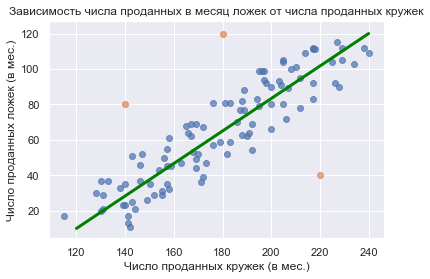
\includegraphics[width=0.54\linewidth]{gr.png}
\end{center}
\begin{enumerate}
	\item Какой вид зависимости Вы наблюдаете? Как это можно объяснить?
	\item Как называется данный вид диаграммы? Как называется зелёная линия? Как называются оранжевые точки? Как называется совокупность синих точек? 
	\item Приведите как минимум один недостаток данного графика (с содержательной точки зрения). 
	\item Верно ли, что в среднем, большинство кружек продавалось, когда число проданных ложек превышало 40? 
\end{enumerate}

\section*{Задание 3: Драконы и зарплаты \\ {\small ВП 2019 – 10 класс 2 этап}}
В Далёкой-Далёкой Стране живут драконы. Они начинают работать в 20 лет и выходят на пенсию в 50 лет. Драконьи учёные провели большой опрос и установили, что зарплата драконов определяется по следующей формуле:
\[
w_i = 20 + 3\cdot(age_i - 20) - 5 \cdot gender_i + 0.5 \cdot gender_i\cdot(age_i - 20),
\]
где:
\begin{itemize}
	\item $w_i$ – годовая (драконы получают зарплату раз в год!) зарплата дракона $i$ (в овцах);
	\item $age_i$ – возраст дракона $i$;
	\item $gender_i$ – пол дракона $i$ (эта переменная равна $0$ для драконов-самцов и $1$ для драконов-самок).
\end{itemize}

Ответьте на следующие вопросы:
\begin{enumerate}
	\item Считая, что драконы работают с одинаковой производительностью независимо от пола, можно ли утверждать, что на их рынке труда присутствует ценовая дискриминация по половому признаку? Аргументируйте свой ответ, используя такие индикаторы, как среднемесячная / среднегодовая заработная плата, которую получает дракон $i$ за весь период своей трудовой деятельности (т.е. с 20 до 50 лет).
	\item Согласно законодательству Далёкой-Далёкой Страны, все виды отпуска, который берут драконы, являются неоплачиваемыми. Как изменится ваш ответ на Пункт 1, если известно, что драконихи уходят в отпуск и уезжают на море на 1 месяц в году, а драконы (самцы) каждый год улетают в экскурсионный тур по достопримечательностям соседних королевств длиной в 3 месяца?
\end{enumerate}

\section*{Задание 4: Доходы \\ {\small ВП 2018 – 10 класс 2 этап}}
При исследовании доходов населения, достаточно часто в экономической литературе можно встретить уравнения следующего рода:
\[
Wage_i = \beta_0 + \beta_1age_i + \beta_2age_i^2 + \ldots
\]
где $Wage_i$ - доход $i$-ого человека, $age_i$ - его возраст, $\beta_0$ , $\beta_1$, $\beta_2$ - коэффициенты, которые
могут быть оценены по реальным статистическим данным. Вместо многоточия может стоять множество других переменных, влияющих на доход.
\begin{enumerate}[label = \alph*)]
	\item Как вы полагаете, зачем в одной модели использовать возраст и квадрат его величины? Какой наблюдающийся в реальности эффект можно описать таким образом?
	\item  Как вы полагаете, какие значения могут принимать переменные $\beta_1$, $\beta_2$ ?
	\item Какие ещё переменные, по Вашему мнению, могут влиять на доход? Для каких из них может быть разумным использование не только самого показателя, но и квадрата этой величины?
\end{enumerate}


\end{document}